\section{Projektmanagement}
Das PREN Modul ist ein Interdisziplinäres Modul. Von jeder der folgenden Fachrichtungen: Informatik, Elektrotechnik und Maschinenbau, ist mindestens eine Person pro Gruppe vertreten. Das Team 27 setzt sich wie folgt zusammen:
\begin{itemize}
	\item 3 Informatiker
	\item 3 Maschinenbauer
	\item 1 Elektrotechniker
\end{itemize}
Anfangs des Moduls wurden den Mitgliedern des Teams verschiedene Funktionen zugewiesen um eine Struktur und Ansprechpersonen innerhalb des Teams zu erhalten. Ersichtlich in folgendem Organigramm:
\begin{figure}[h!]
	\centering
	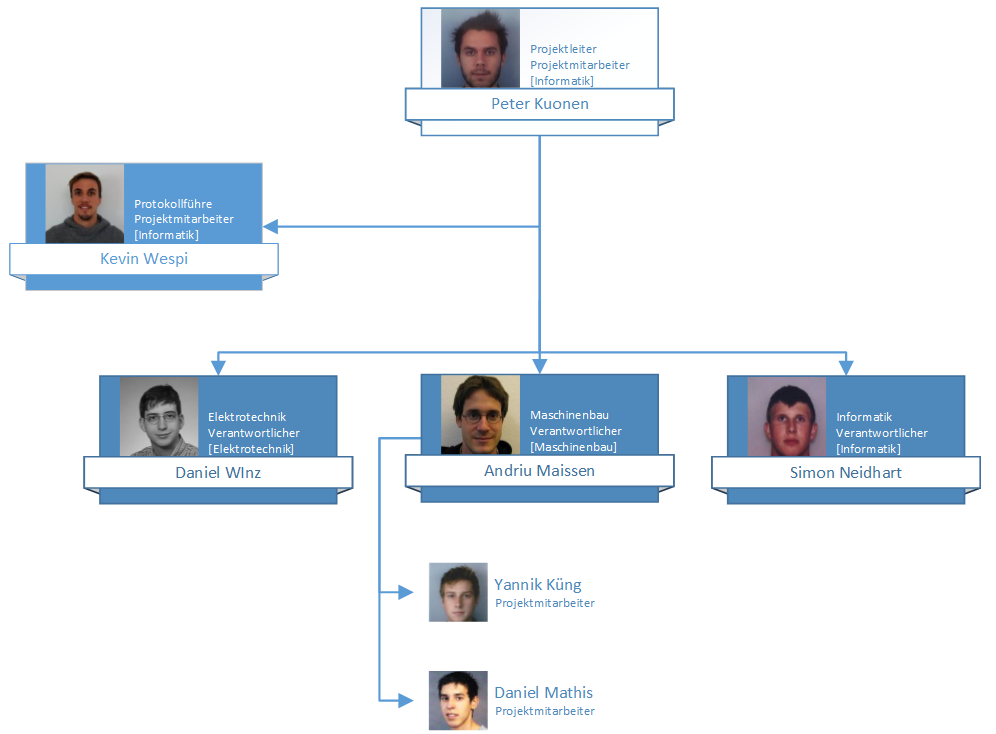
\includegraphics[width=0.7\textwidth]{fig/Organigramm.png}
	\caption{Organigramm}
	\label{fig:Organigramm}
\end{figure}

\subsection{Projektplanung}
Im folgenden wird die Planung mittels Zeitachsen für die jeweiligen Meilensteine dargestellt. In den folgenden Abbildungen sind diese dargestellt. Sie enthalten die Hauptaufgaben welche für die jeweiligen Meilensteine notwendig sind. Dies wurde angefertigt um die Übersicht über das Projekt zu haben und die verlangten Dokumente und Schritte zur Erfüllung der Meilensteine fristgerecht zu erledigen.

\begin{figure}[h!]
	\centering
	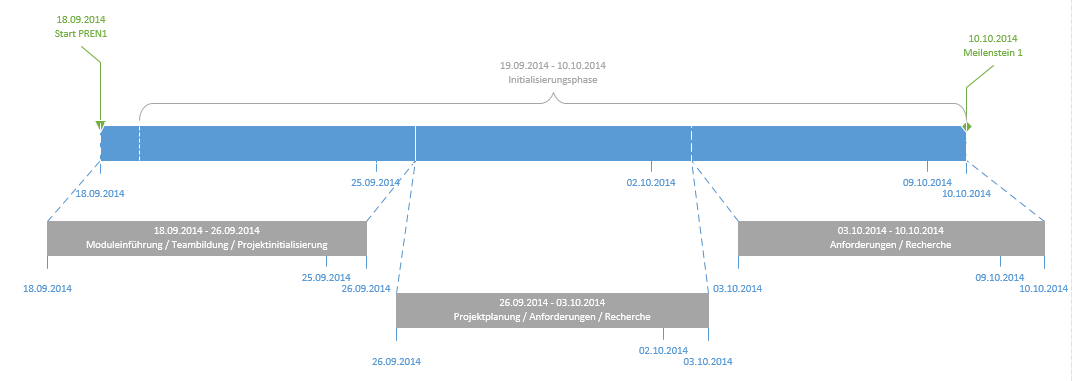
\includegraphics[width=1\textwidth]{fig/PlanungBisMS1.png}
	\caption{Planung Meilenstein 1}
	\label{fig:MS1}
\end{figure}
\begin{figure}[h!]
	\centering
	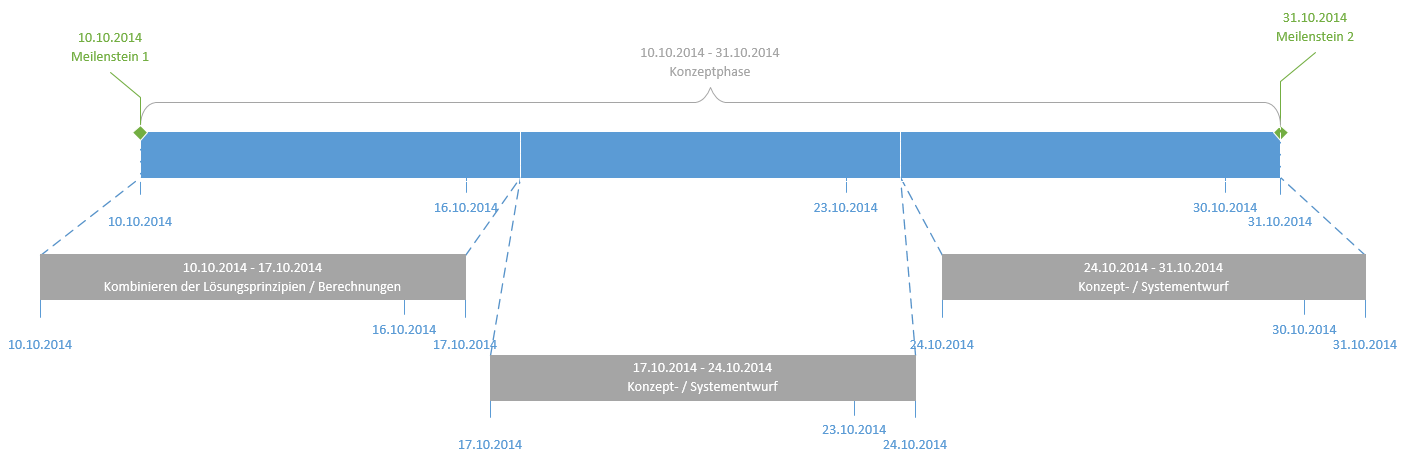
\includegraphics[width=1\textwidth]{fig/PlanungBisMS2.png}
	\caption{Planung Meilenstein 2}
	\label{fig:MS2}
\end{figure}
\begin{figure}[h!]
	\centering
	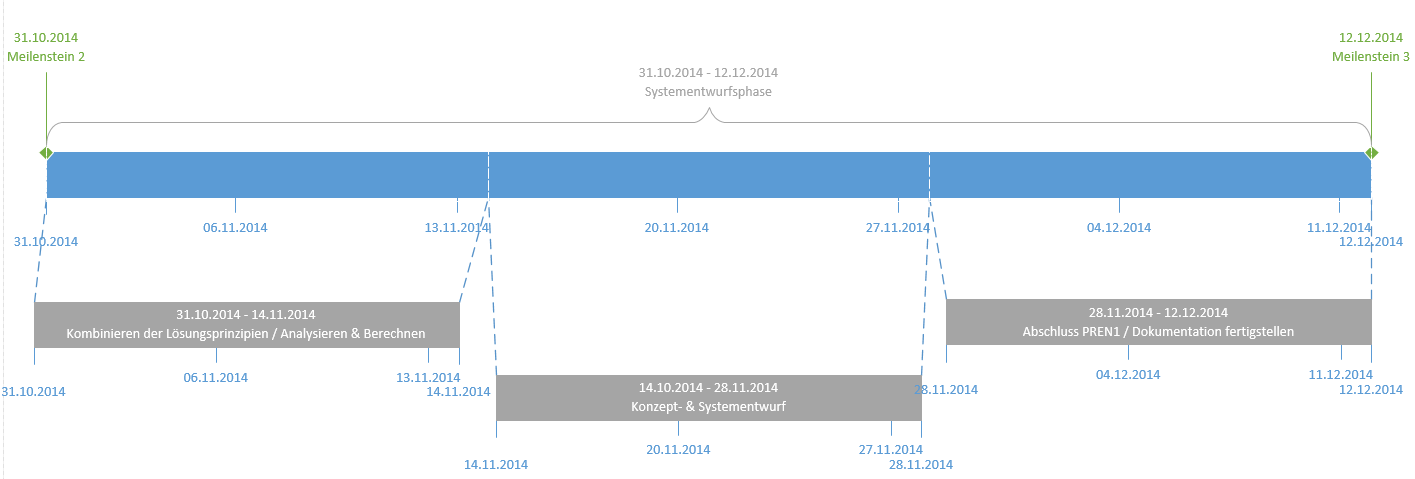
\includegraphics[width=1\textwidth]{fig/PlanungBisMS3.png}
	\caption{Planung Meilenstein 3}
	\label{fig:MS3}
\end{figure}
\newpage
%\begin{landscape}

\subsection{Risikoanalyse allgemein}
Bevor das Projekt richtig gestartet wird, soll eine allgemeine Risikoanalyse erstellt werden. Das Team hat sich Gedanken darüber gemacht, was schief gehen kann und wie man mit den erkannten Problemen umgehen oder ihnen vorbeugen kann. Zudem wurde die Wahrscheinlichkeit und die Auswirkung der eruierten Probleme notiert. Mit der Liste im Hinterkopf wird das Projekt mit einem anderen Mindset angegangen und Fehlerquellen werden minimiert. 

\begin{table}[h!]
	\begin{zebratabular}{@{}cp{0.25\linewidth}llp{0.25\linewidth}}		
		\textbf{ID}&\textbf{Beschreibung}&\textbf{Wahrscheinlichkeit}&\textbf{Auswirkung}&\textbf{Massnahmen}\\
		\hline
		\#1&Teammitglied Elektrotechnik fällt aus&sehr niedrig&sehr hoch&keine\\
		\#2&Teammitglied Maschinenbau fällt aus&sehr niedrig&hoch&Übernahme durch Maschinenbauer\\
		\#3&Teammitglied Informatik fällt aus&sehr niedrig&hoch&Übernahme durch Informatiker\\
		\#4&Budget wird überschritten&niedrig&hoch&Vorab Kosten abklären\\
		\#5&Zeit reicht nicht zur Realisierung&mittel&sehr hoch&Zeitplanung mit Meilensteinen\\
		\#6&Eingekaufte Komponente fällt aus&niedrig&hoch&Neu bestellen\\
		\#7&Komponente (Eigenbau) fällt aus&niedrig&mittel&Neu bauen\\
		\#8&Komponente funktioniert nicht&niedrig&mittel&Komponente reparieren\\
		\#9&Berechnungen falsch&sehr niedrig&hoch&Überprüfung durch mehrere Personen\\
		\#10&Abmessungseinschränkungen überschritten&sehr niedrig&hoch&Modell bauen\\
		\#11&Schnittstellen ungenau definiert&sehr niedrig&sehr hoch&Überprüfung durch mehrere Personen\\
		\#12&Startsignal funktioniert nicht&niedrig&hoch&Ausgiebiges Testen\\
		\#13&Endsignal nicht übermittelt&niedrig&sehr niedrig&Ausgiebiges Testen\\
		\#14&Verfehlen des Korbs&mittel&mittel&Ausgiebiges Testen\\
		\#15&Stromversorgung reicht nicht aus&sehr niedrig&mittel&Ausgiebiges Testen\\
		\#16&Anforderungen ändern&sehr niedrig&hoch&Neu planen\\
	\end{zebratabular}
\end{table}
%\end{landscape}
